

% should i preface the reader with the reason for the background?
% what is the reason for the background?
The lolly machine is comprised of many different components from pneumatic actuators to industrial communication protocols - most of which do not come under the banner of common knowledge. The background section aims to preface the reader with all necessary information required to understand all components, hence allowing the reader to comprehend the work that has been completed. 

\section{Pneumatics}
    Pneumatics is a category of mechanical engineering  where air flow is converted into mechanical energy\cite{parr2011hydraulics}. The mechanical energy is then used to do work. A typical application of pneumatics is to move an actuator from one position to another, i.e. from open to closed. Pneumatics are common within the food processing industry as a malfunction within the system will not spoil the product.
    All mechanical movement within the lolly machine is driven by pneumatic actuators.
    
\section{Linear Actuators}
    Linear actuators, as the name suggests, provides linear movement to push and/or pull objects within a given process. The linear actuators on the lolly machine are powered by pneumatics. The main components of a linear actuator are as follows:
    
    \begin{description} 
        \item\textbf{Rod:} connects the actuator to the outside environment.
        \item\textbf{Piston:} facilitates movement to the rod through applied pressure to either side.
        \item\textbf{Barrel:} houses the piston.
        \item\textbf{Extend Port:} when air enters, the rod will extend outwards.
        \item\textbf{Retract Port:} When air enters, the rod will retract inwards.
    \end{description}
    
    The fundamental concept is that the differential pressure between either side of the piston will cause it to move\cite{parr2011hydraulics}. The direction of movement is dependent on the flow of air through the extend and retract ports.
    
    
    There are eight linear actuators installed on the lolly machine. Three are used within the sorting process while five are required for dispensing. Figure \ref{fig:rejectAct} shows the linear actuator responsible for dropping lollies into the colour sensing shoot.

    \begin{figure}[H] 
        \centering
        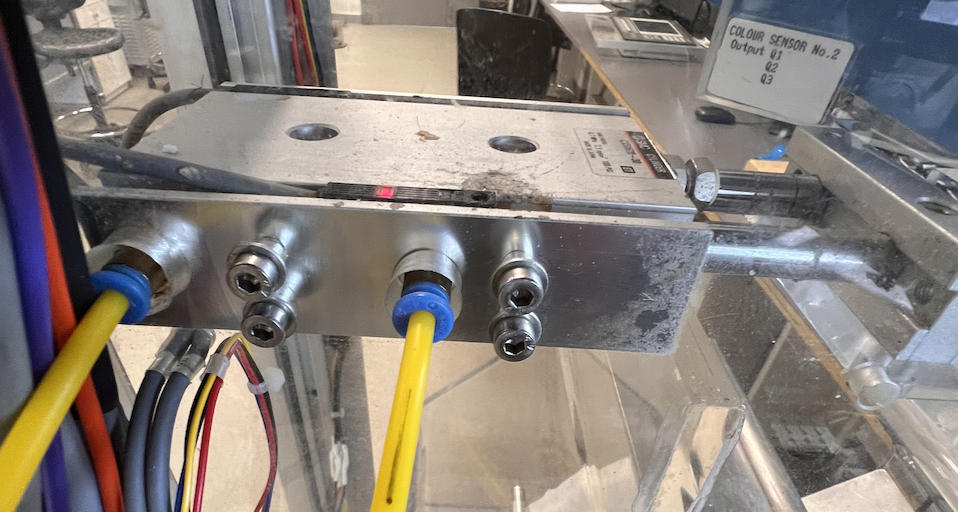
\includegraphics[width = 0.5\textwidth]{2_images/rejectAct.png}
        \caption{Lolly machine reject actuator.}
        \label{fig:rejectAct}
    \end{figure}        
    
\section{Rotary Actuators}
    Rotary actuators provide rotational movement to objects through a central shaft\cite{parr2011hydraulics}. Rotation can be restricted or unrestricted. A rack and pinion or vanes facilitate the turning action within the actuator\cite{parr2011hydraulics}. Rotary actuators within the lolly machine are driven by a single vane and restricted to 90$^{\circ}$\cite{smcRot}. There are three rotary actuators installed on the lolly machine.

\section{Pneumatic Control Valves}
    The pneumatic control valves on the lolly machine, manage air flow to pneumatically driven actuators. Pneumatic control valves are defined by the number of ports, positions, and their control action\cite{parr2011hydraulics}. Figure \ref{fig:controlValves} compares two different types of valves - (a) shows a four-port two-position valve (4/2) while (b) shows a four-port, 3-position valve(4/2). Figure \ref{fig:controlValveConfig} shows a possible internal configuration for the 4/3 valve. It is important to note that the above mentioned figures do not represent typical pneumatic valve symbols and are included to illustrate the differences between various types of control valve configurations.
    
    \begin{figure}[H]
    \centering
    \begin{minipage}{0.45\textwidth}
        \centering
        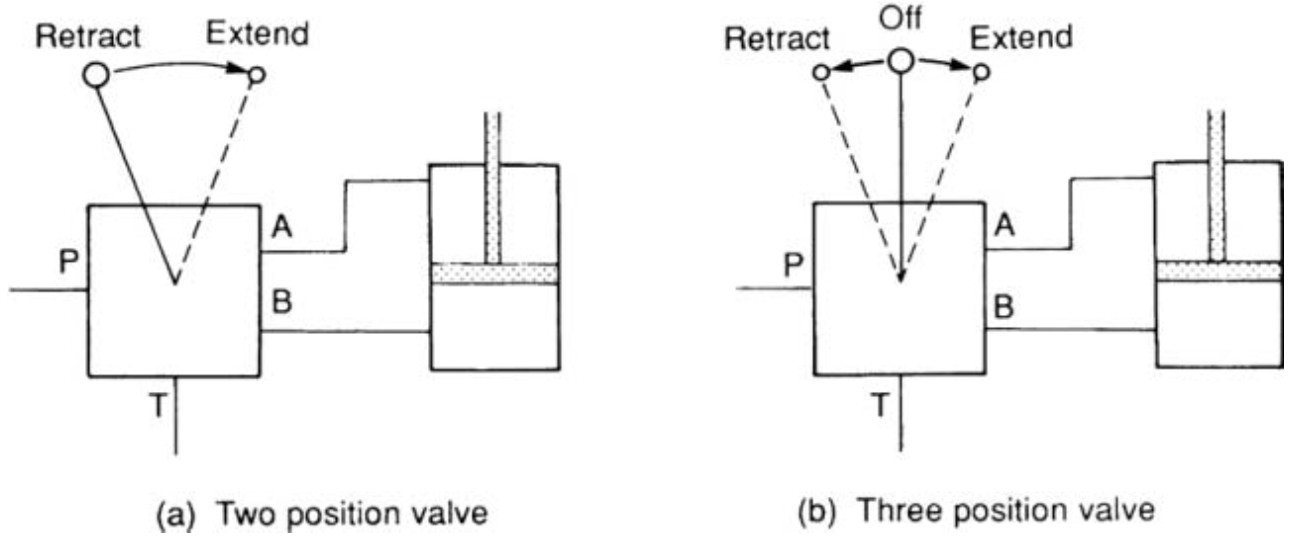
\includegraphics[width = 1\textwidth]{2_images/controlValves.png}
        \caption{Comparison between control valves~\cite{parr2011hydraulics}.}
        \label{fig:controlValves}
    \end{minipage}\hfill
    \begin{minipage}{0.5\textwidth}
        \centering
        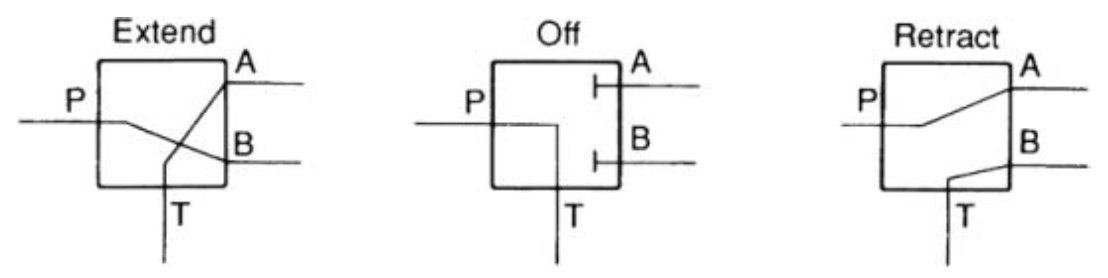
\includegraphics[width = 1\textwidth]{2_images/controlValveConfig.png}
        \caption{4/3 control valve switching configuration~\cite{parr2011hydraulics}.}
        \label{fig:controlValveConfig}
    \end{minipage}\hfill            
    \end{figure}      

    All actuators on the lolly machine are driven by 5/2 control valves, this means that each valve has two positions and 5 ports. Figure \ref{fig:5_2Valve} shows a 5/2 pneumatic valve symbol. Valve positions are shown by two square boxes (coloured red and green to clearly illustrate the different positions) each containing two arrows and a T. The arrows show the air flow direction between ports while the T represents a plug. The zigzag on the right hand side of the symbol illustrates a spring, indicating the the control valve is spring return. The rectangle with the diagonal line through the middle shows that a solenoid drives the control action. Figure \ref{fig:cylinderAB} shows the two possible positions of the cylinder.

    \begin{figure}[H]
    \centering
    \begin{minipage}{0.45\textwidth}
        \centering
        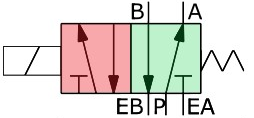
\includegraphics[scale = 0.5]{2_images/5_2Valve.png}
        \caption{A 5/2 pneumatic control valve \cite{5_2Valves}.}
        \label{fig:5_2Valve}
    \end{minipage}\hfill
    \begin{minipage}{0.5\textwidth}
        \centering
        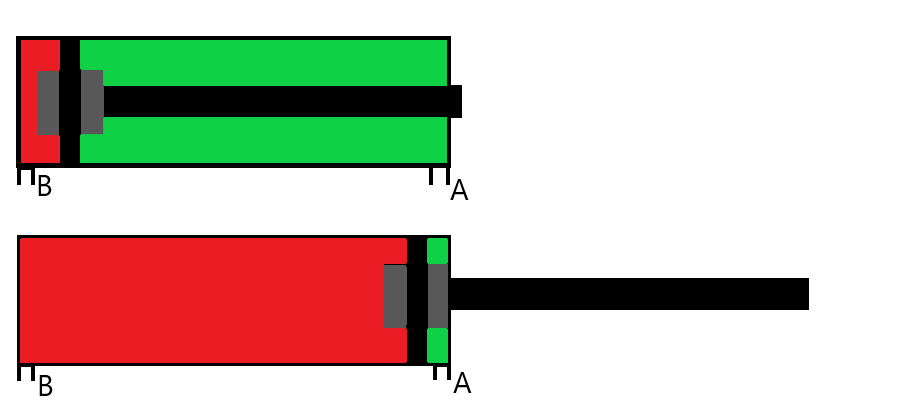
\includegraphics[width = 0.8\textwidth]{2_images/cylinderAB.png}
        \caption{Different cylinder positions. \\Position 1(Top) = Retracted. \\Position 2(Bottom) = Extended}
        \label{fig:cylinderAB}
    \end{minipage}\hfill            
    \end{figure}          
   
   The below position descriptions are in reference to Figure \ref{fig:5_2Valve}.
    \begin{description}
        \item\textbf{Position 1 - Green:}
        While the valve is in position 1 the pressure (P) port is connected to the (A) port and (B) port is connected to the exhaust line (EB).
        \item\textbf{Position 2 - Red:}
        While the valve is in position 2 the pressure (P) port is connected to the (B) side and (A) port is connected the exhaust line (EA). 
    \end{description}
    
    The control action is what triggers the pneumatic control valve and can vary depending on the application, typical control actions include\cite{parr2011hydraulics}:
    \begin{itemize}
        \item Push Button
        \item Spring
        \item Lever
        \item Roller Limit Switch
        \item Pressure Line
        \item Solenoid
    \end{itemize}
    
    All control valves on the lolly machine are are triggered via solenoid driven pilot valves.

\section{I/O}
    
    \acrfull{io}, as the name suggests, are the inputs and outputs of a control system. Inputs are often referred to as sensors as they are devices that translate a real world signal into something that the \acrshort{cpu} can make sense of - this typically consists of some sort of electrical signal (Voltage or Current). Outputs, on the other hand, are often referred to as "final control elements" or "actuators". Output devices are how the control system is able to interact with the outside world.\\
    There are four main types of \acrshort{io}:

    \begin{description}
    \item\textbf{Digital Inputs} - Binary input signals (On or Off).
    \item\textbf{Digital Outputs} - Binary output signals (On of Off).
    \item\textbf{Analog Inputs} - Variable electrical (voltage or current) inputs signals.
    \item\textbf{Analog Outputs} - Variable electrical (voltage or current) output signals.
    \end{description}
    
    The lolly machine \acrshort{io} is comprised of digital inputs and outputs. This section will provide a brief overview to all different types of digital \acrshort{io} that can be found on the lolly machine

\subsection{Inputs}
    \subsubsection{Limit Switches}
        Magnetically activated limit switches manufactured by \acrshort{smc} provide actuator position feedback. There are two limit switches installed on each actuator, one that activates when the actuator is fully extended and the other when it is fully retracted. The limit switches are installed within a track on the actuator and held in place by a small grub screw - this can be seen in Figure \ref{fig:rejectAct}.
        The limit switches have an internal solid state circuit that is activated when the piston is adjacent. The piston is made from a magnetic ferrous material which is what allows the switch to activate. 
        Figure \ref{fig:autSwShm} shows the internal electrical schematic of the \acrshort{smc} limit switches.
        
        \begin{figure}[H]
            \centering
            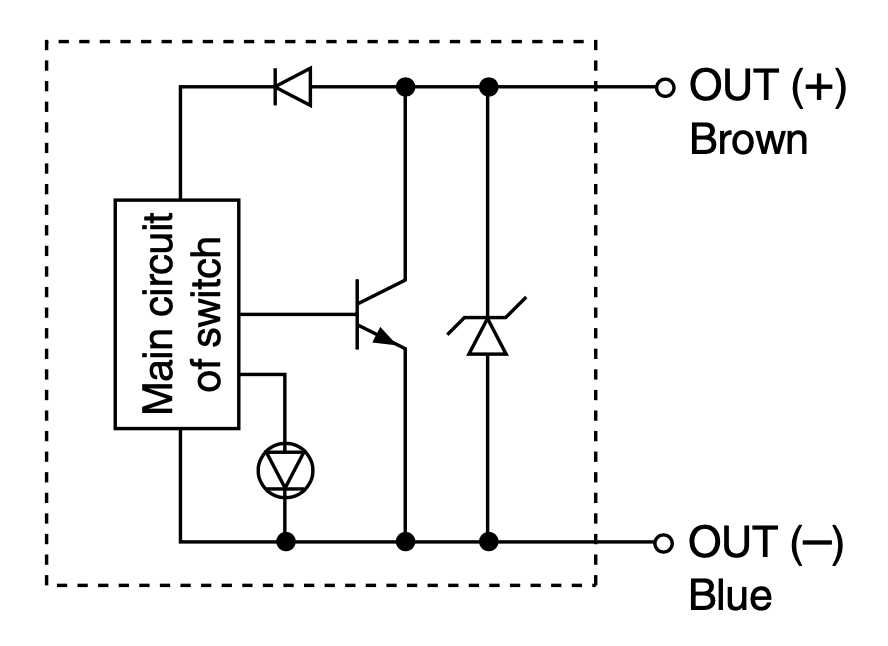
\includegraphics[scale = 0.4]{2_images/autSwShm.png}
            \caption{Internal electrical schematic of an \acrshort{smc} limit switch~\cite{smcRot}.}
            \label{fig:autSwShm}
        \end{figure}

    \subsubsection{Proximity Sensors}
        Two proximity sensors are installed on the lolly machine. The sensors determine whether or not a lolly is in situ. The proximity sensors installed on the lolly machine are capacitive; this allows the sensors to detect ferrous and non-ferrous materials. Figure \ref{fig:proxSens} illustrates the general function of a proximity sensors. In the case of the lolly machine, the proximity sensors are \acrshort{nc} which means that the output is on when the target is detected and off while the target is not.
    \begin{figure}[H]
    \begin{minipage}{0.35\textwidth}
        \centering
            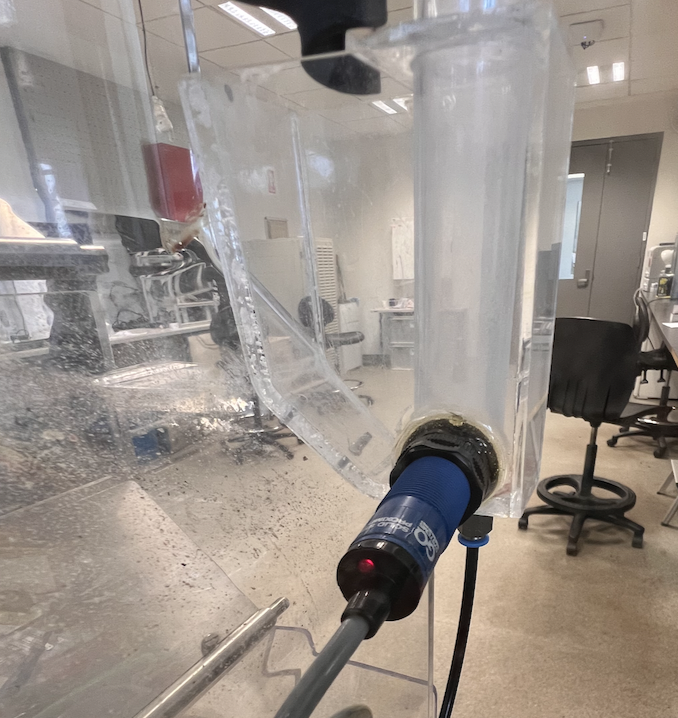
\includegraphics[scale = 0.4]{2_images/rejectProx.png}
            \caption{Lolly machine proximity sensor used to detect when a lolly is in the reject bucket.}
            \label{fig:rejectProx}
    \end{minipage}\hfill
    \begin{minipage}{0.35\textwidth}
        \centering
        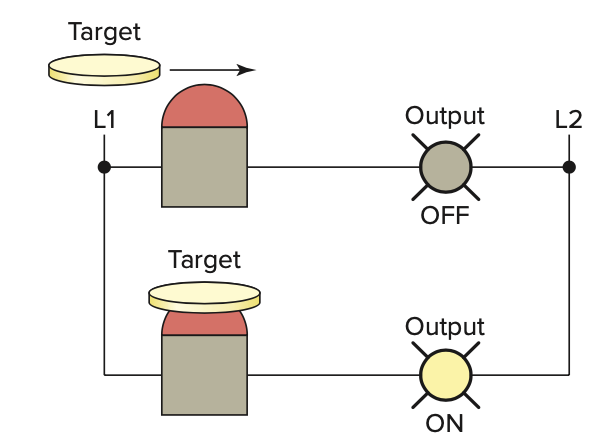
\includegraphics[width = 0.9\textwidth]{2_images/proxSens.png}
        \caption{Typical function of a proximity sensor \cite{petruzella2017programmable}.}
        \label{fig:proxSens}
    \end{minipage}\hfill 
    \end{figure}
    
    \subsubsection{Colour Sensors}
        The colour sensors onboard the lolly machine emit Red, Green and Blue light onto each passing lolly, the radiation reflected off the lollies is detected and compared to previously stored/ learned coordinates within the sensor \cite{sickColourSenors}. If the detected radiation of the lolly is within a certain tolerance of the learned coordinates then an output from the sensor is set to true, indicating that a desired colour has been detected. There are two "SICK" colour sensors on-board the lolly machine - one that can detect three different colours while the other, only one.
        %Although the colour sensors used on the lolly machine can’t actually detect the complete range of colours which can be seen by us, the two colours sensors (3 digital signals from one sensor, and 1 digital signal from the second), are able to be “trained/calibrated” to provide an indication of a number of different colour matches.
        Figure \ref{fig:cs1} shows the electrical connections of one of the colour sensors while Figure \ref{fig:colSens} shows a picture of the colour sensors installed on the machine.

        \begin{figure}[H]
            \centering
            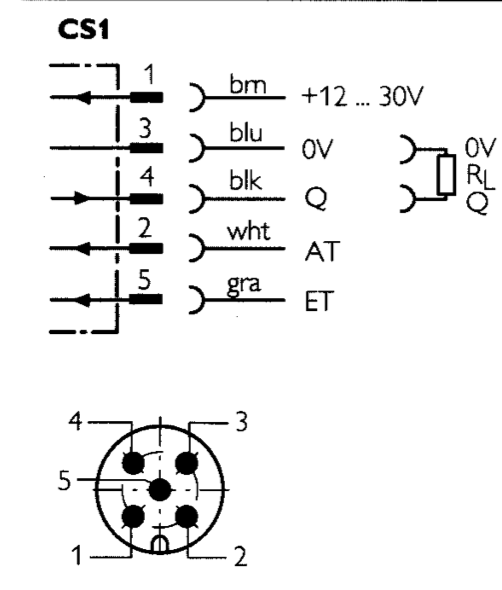
\includegraphics[scale = 0.4]{2_images/cs1.png}
            \caption{Electrical connections for a single output colour sensor \cite{sickCs}.}
            \label{fig:cs1}
        \end{figure}     
        
        \begin{figure}[H]
            \centering
            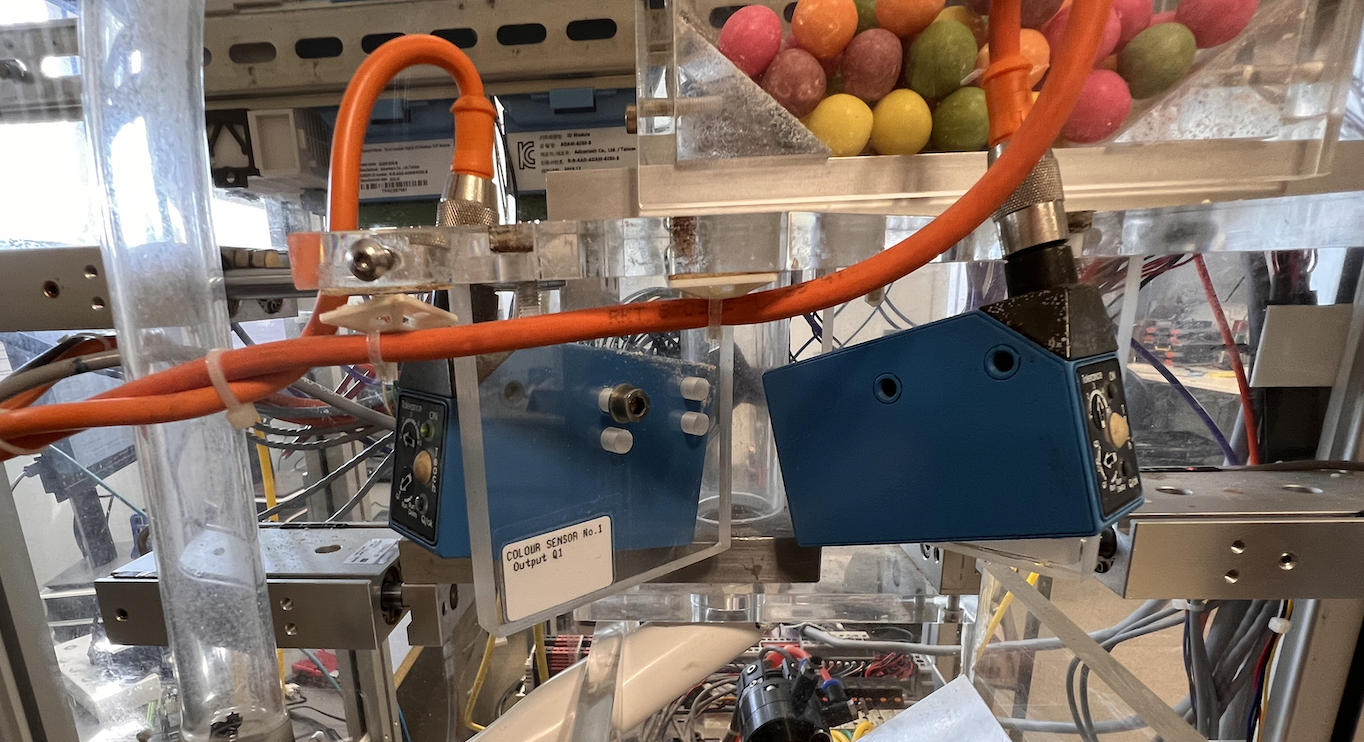
\includegraphics[scale = 0.4]{2_images/colSens.png}
            \caption{The two lolly machine colour sensors.}
            \label{fig:colSens}
        \end{figure}       

    \subsubsection{Buttons}
    Physical push buttons provide an interface between the operator and the machine where different buttons are linked to different machine functions. For example, an \acrfull{estop}, when pressed, will halt the operation of the machine and put it into error mode. While in error mode, the machine will cease to operate until it has been an given instruction by the user that it is safe to do so. The \acrshort{estop} is a \acrshort{nc} contact while the rest of the buttons on the machine are \acrshort{no}.
    %Find a figure of a NO button - can probably find in the PLC book
    
\subsection{Outputs}
    \subsection{Solenoids - Pneumatic Valve}
    All pneumatic actuators on the lolly machine are activated by pneumatic control valves. The control valves are activated by an internal solenoid driven pilot valve.  The output device, from the perspective of the \acrshort{plc}, is the solenoid. The fundamental components of a solenoid are a wire coil and ferrous core. The ferrous core is located within the coil. When a \acrshort{dc} voltage is applied to the coil it behaves like a magnet, this is called an electromagnet. When the solenoid is switched, the ferrous core moves from one end of the solenoid housing to the other. The core is connected to the pilot valve which provides the necessary mechanical action to change the valve position, which in turn, moves the actuator. 
    
        \begin{figure}[H]
            \centering
            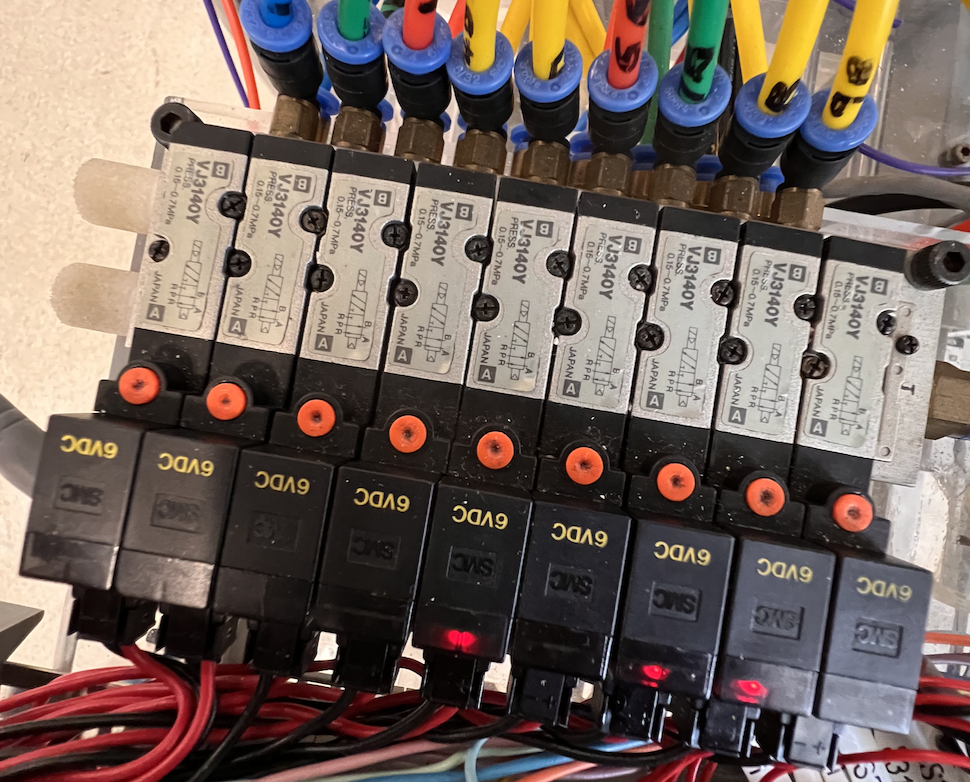
\includegraphics[scale = 0.5]{2_images/controlValvesPic.png}
            \caption{Solenoid pneumatic control valves mounted on manifold.}
            \label{fig:controlValvesPic}
        \end{figure} 
    
    \subsubsection{\acrshort{led} Indicators}
        A number of \acrshort{led} based lights are used on the lolly machine. The \acrshort{led}s are linked to specific machine states and will either be on, off  or flashing. \acrshort{led}s are robust, lasting much longer than previously used incandescent lights. As most \acrshort{led}s require only a couple of volts, all have internal series resistors which allows all \acrshort{led}s on the lolly machine to be directly controlled and switched by the \acrshort{plc}.
        
        \begin{figure}[H]
            \centering
            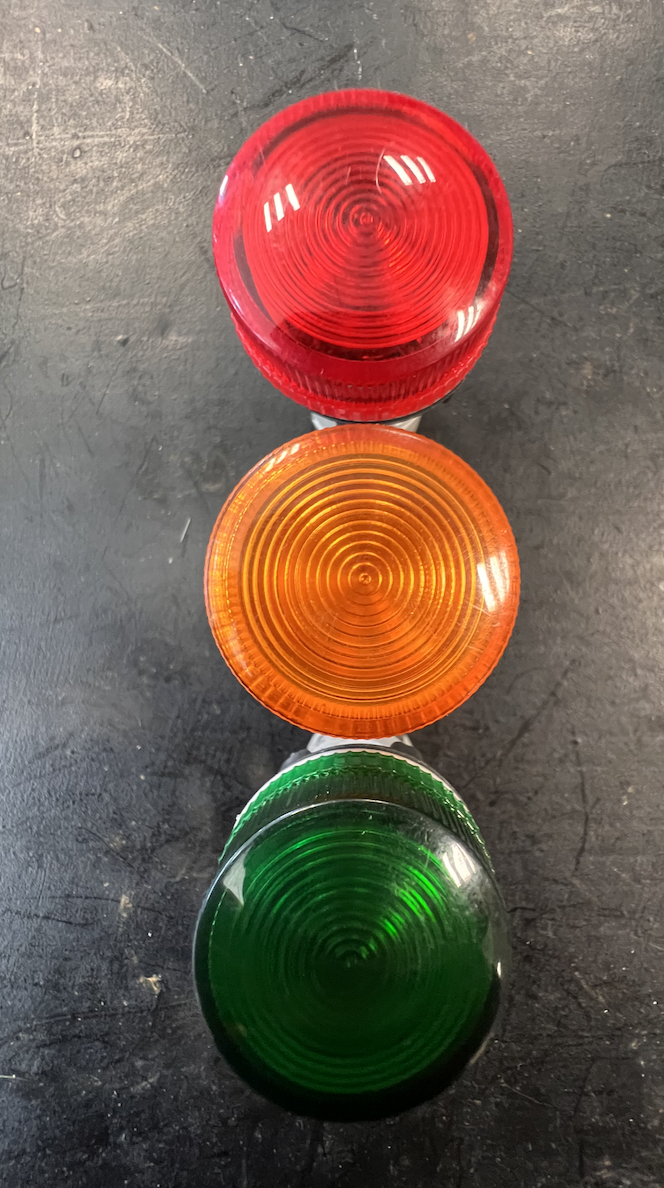
\includegraphics[scale = 0.3]{2_images/leds.png}
            \caption{Lolly machine \acrshort{led}s}
            \label{fig:leds}
        \end{figure} 
        
%There are two main streams of process control - continuous and sequential\cite{dunn2006introduction}. Continuous control involves the constant monitoring and manipulation of dynamic systems while while sequential control is event based. Given the nature of the lolly machine, sequential control is the obvious choice for controlling the system \cite{dunn2006introduction}.

The lolly machine is, in essence, an automatic machine. This section investigates various components that facilitate the automation aspects of the project.

\section{State Machine Design}
    State machine design, sometimes refereed to as sequential machine design, is a systematic method of programming which is commonly used to structure and machine code. Different variations of state machine design exist within industry and sometimes they can be difficult to identify, making the code look unnecessarily complicated and confusing to read. State machine design is comprised of different states with transitions between states. Actions within each state define how the machine will behave in said state while transitions between states are the conditions than need to exist to allow the machine to transition from one state to another. Figure \ref{fig:stateMachineEx} shows the general concept of state machine design. State machine design can be written in arguably any language. Some languages, like GRAPH by Siemens, are based on the concept of state machine design as evident by the look and feel of the language\cite{siemensGraph}. 

    \HD{If you get time - find a reference that backs up what you have said here about state machine design}

        \begin{figure}[H]
        \centering
        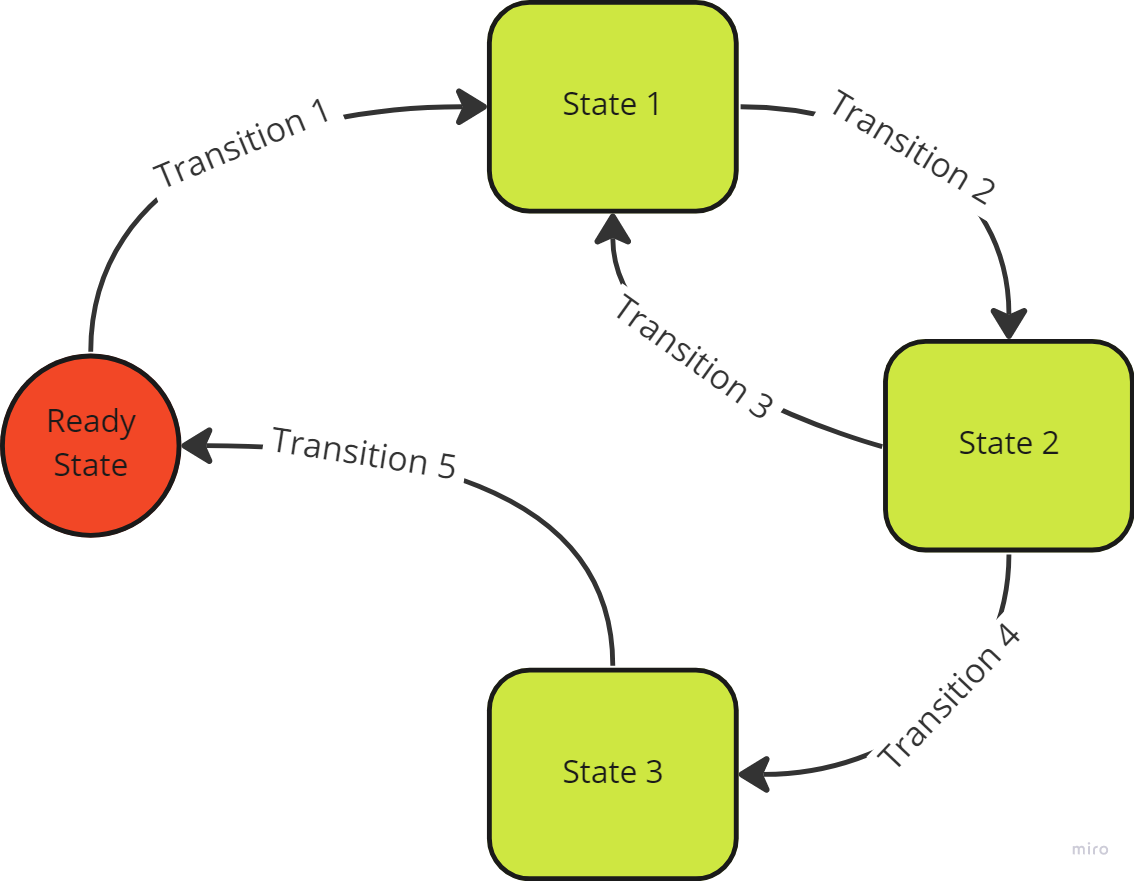
\includegraphics[width = 0.5\textwidth]{2_images/stateMachineEx}
        \caption{The general concept behind state machine design.}
        \label{fig:stateMachineEx}
    \end{figure}

\section{Programmable Logic Controller (PLC)}


    A \acrfull{plc} is an industrial controller/ computer that can be programmed to perform specific \acrshort{rt} tasks and can utilised for varying applications\cite{petruzella2017programmable}. A \acrshort{plc} performs these tasks through solving logic based operations\cite{petruzella2017programmable}.  E.g., if a water tank is filled to a level which is deemed "to high" turn off the water supply to the tank. A \acrshort{plc} interacts with the outside world through the use of either onboard or remote \acrshort{io}.
    
    Prior to the existence of \acrshort{plc}s, sequential based control was performed through relay\footnote{Relays are an electrical component comprised of a solenoid and contacts(\acrshort{no} and/or \acrshort{nc}), when the solenoid is energised the contacts change state.}-logic. Relay logic required multiple relays to be wired in a certain configuration allowing for the control of the system. Figure \ref{fig:relayLogic} shows an example of a relay-logic based control system\cite{petruzella2017programmable}. 
    \acrshort{plc}s provided a much cleaner, organised and easier to troubleshoot method of control as seen in Figure \ref{fig:plcLogic}.    
    
    \begin{figure}[H]
    \centering
    \begin{minipage}{0.35\textwidth}
        \centering
        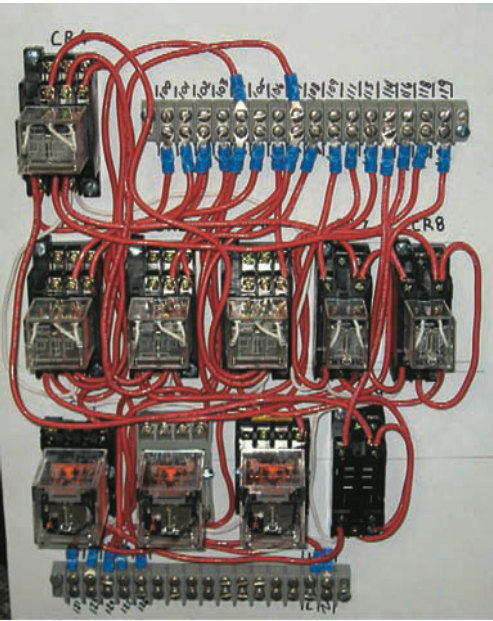
\includegraphics[width = 0.9\textwidth]{2_images/relayLogic.png}
        \caption{Relay logic based control system.~\cite{petruzella2017programmable}}
        \label{fig:relayLogic}
    \end{minipage}\hfill
    \begin{minipage}{0.35\textwidth}
        \centering
        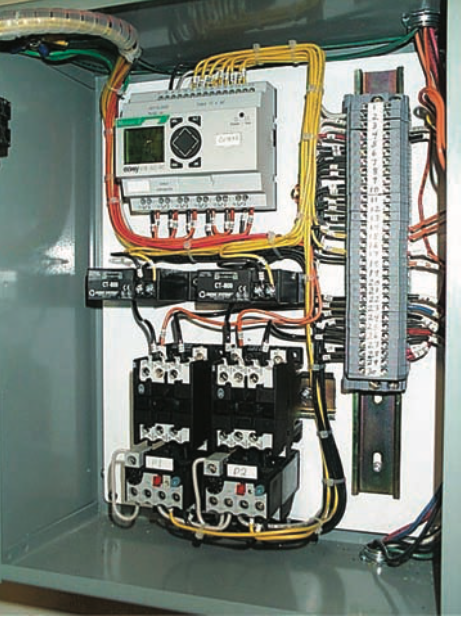
\includegraphics[width = 0.9\textwidth]{2_images/plcLogic.png}
        \caption{\acrshort{plc} based control system.~\cite{petruzella2017programmable}}
        \label{fig:plcLogic}
    \end{minipage}\hfill            
    \end{figure}   
    
    Originally, \acrshort{plc}s where exclusively programmed in a language called \acrfull{ld}\cite{petruzella2017programmable}. Ladder logic is a visual programming language based on electrical control schematics and was designed to be used by the same people who were building the relay logic based control systems ,electricians\cite{petruzella2017programmable}. In more recent times \acrshort{plc}s have become more sophisticated and can be programmed in a variety of languages including \acrfull{st} which is a text based language\cite{petruzella2017programmable}. 
    
    A \acrshort{plc}'s main components are a power supply, \acrlong{cpu}, and \acrshort{io} modules. \acrshort{io} modules can be located locally or remotely. Local \acrshort{io} is physically connected to the \acrshort{plc} while remote \acrshort{io} is connected to the \acrshort{plc} via a communication line, this is illustrated in Figure \ref{fig:localRemoteIo}.
       
    \begin{figure}[H]
        \centering
        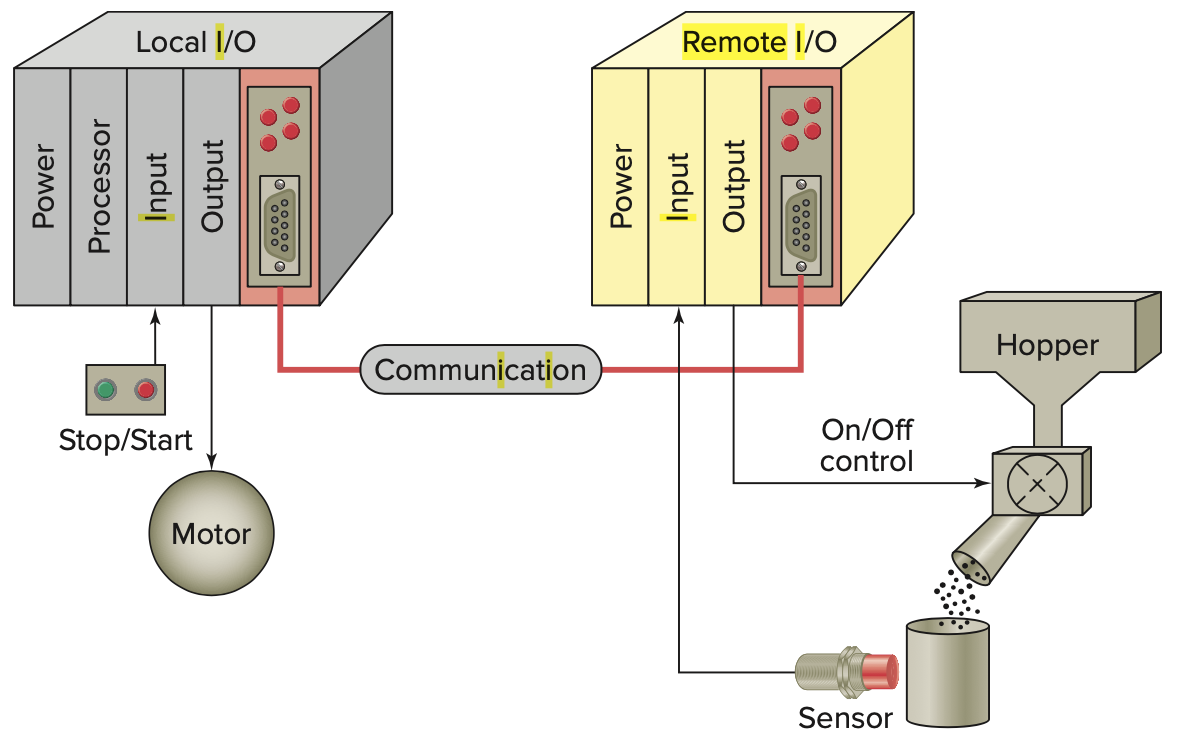
\includegraphics[width = 0.5\textwidth]{2_images/localRemoteIo.png}
        \caption{Local and remote \acrshort{io}}
        \label{fig:localRemoteIo}
    \end{figure}
 
\section{Human Machine Interface (HMI)}
    A \acrfull{hmi}, as the name suggests, is the interface between the machine and the human/ operator. A \acrshort{hmi} is a screen that shows the machine state through graphics. An operator enters commands through the touch screen or a keyboard and mouse. \acrshort{hmi}s are programmable and can be used to control and monitor almost any machine\cite{petruzella2017programmable}. Typically, there is one \acrshort{hmi} per machine/ operator. It is not uncommon to have multiple \acrshort{hmi}s within a single factory. Figure \ref{fig:typHmi} shows an example of what a \acrshort{hmi} screen for a basic motor controller might look like.

    \begin{figure}[H]
        \centering
        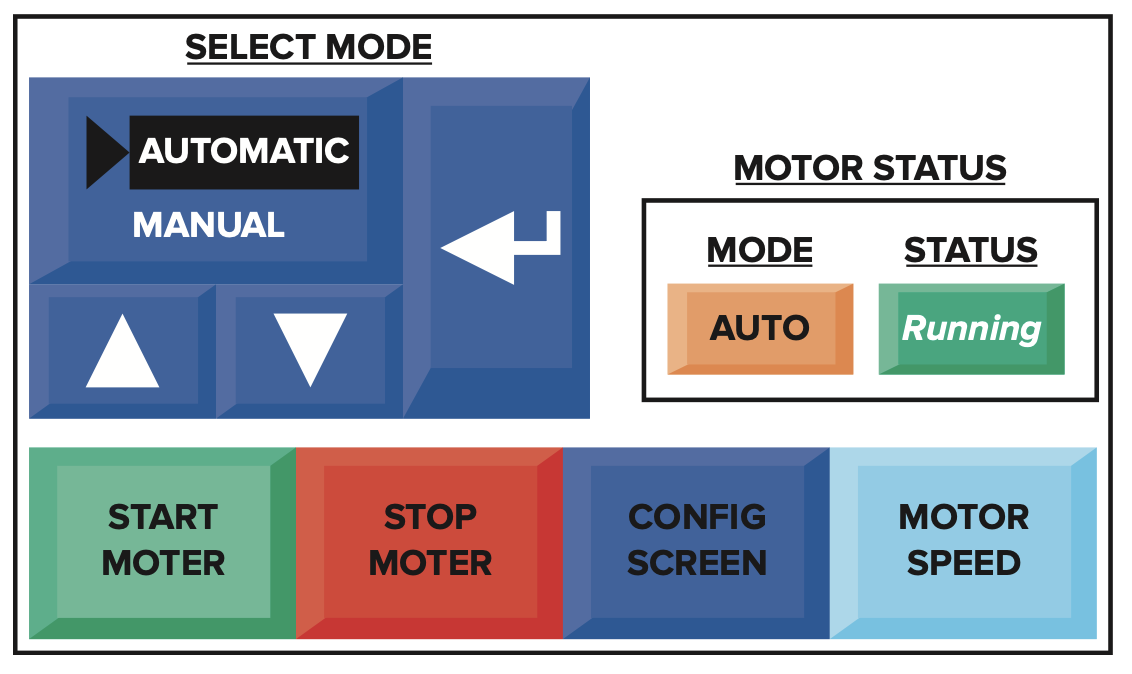
\includegraphics[width = 0.5\textwidth]{2_images/typicalHmi.png}
        \caption{A typical \acrshort{hmi} motor controller screen\cite{petruzella2017programmable}}
        \label{fig:typHmi}
    \end{figure}    
    
\section{Engineering Workstation}
    An engineering workstation is a \acrshort{pc} that has been set up for a engineer. The engineering workstation is connected to the \acrshort{ot} network and setup with all relevant software specific to the controlled process. In the case of the lolly machine the engineering workstation is a desktop computer that has all of the necessary  software to connect, configure and program all system hardware. 
\section{Microcontrollers}
    To understand what a microcontroller is, a few definitions must be made \cite{crisp2003introduction}.
    
\begin{description}
    \item{\textbf{Integrated Circuits:}} - An electronic circuit that is printed onto solid block. The circuit contains semi-conductor components. Integrated circuits are often referred to as chips.
    \item{\textbf{Microprocessor:}} - A microprocessor is part of a system, it is the central processing unit and is useless without surrounding circuitry and applied voltages.
    \item{\textbf{Microprocessor-based System:}} A microprocessor-based System is any system that is controlled by a microprocessor. 
\end{description}    
    
    A \textbf{microcontroller} is a microprocessor-based embedded system built into an integrated circuit and is usually capable of controlling its own \acrshort{io} \cite{crisp2003introduction}.
    
    Microcontrollers are capable of performing an almost infinite list of tasks, e.g., controlling a wrist watch, monitoring and controlling a home irrigation system or controlling a robot. Some micorcontrollers, like the ones in a wrist watch or calculator,  can not be easily programmed after they leave the factory while other can.
    
    Similar to a \acrshort{plc}, micorcontrollers have onboard \acrshort{io} with the caveat being the hyper sensitivity to voltages above the standard operating voltage of the microcontroller which is typically 3.3 volts. Two micorcontrollers are used on the lolly machine - these are a Raspberry Pi and an Arduino.  
  
    \begin{figure}[H]
    \centering
    \begin{minipage}{0.4\textwidth}
        \centering
        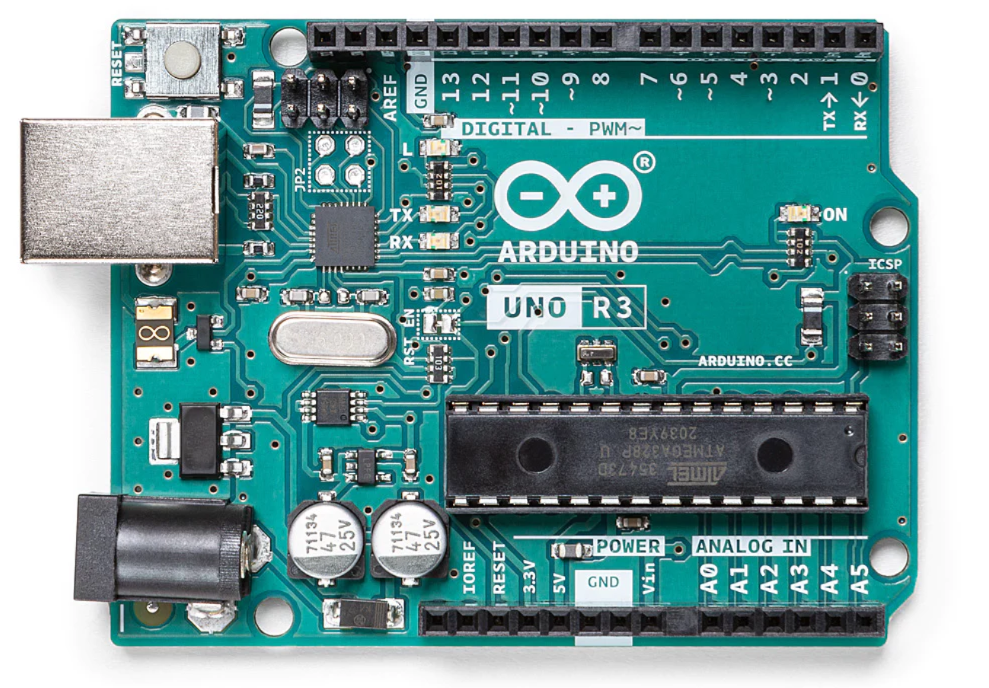
\includegraphics[width = 0.8\textwidth]{2_images/arduino.png}
        \caption{An Arduino~\cite{arduinoWeb}}
        \label{fig:arduino}
    \end{minipage}\hfill
    \begin{minipage}{0.4\textwidth}
        \centering
        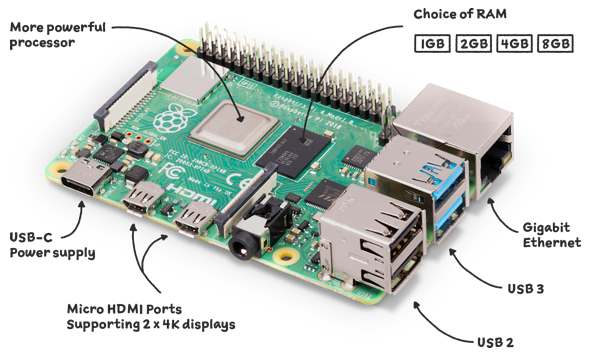
\includegraphics[width = 0.9\textwidth]{2_images/RaspPi.png}
        \caption{A Raspberry Pi~\cite{raspPiWeb}}
        \label{fig:raspPi}
    \end{minipage}\hfill            
    \end{figure}     

\subsection{Data Types}
    Data types represent different numerical formats within a process control system. Most variables within the lolly machine are Boolean (bit). The below list defines the basic data types used within a process control system. 
    
    \begin{table}
    \centering
    \caption{Data types of a typical control system.}
        \begin{tabular}{ |p{3cm}|p{2cm}|p{3cm}|  }
                \hline
                \multicolumn{3}{|c|}{\textbf{Data Types}} \\
                \hline
                \textbf{Type}& \textbf{Bits}& \textbf{Example} \\
                \hline
                Bit & 1 & True/False or 1/0 \\
                Byte & 8 & 16\#8 or 00001000 \\
                Word & 16 & 16\#F8 \\
                Double Word & 32 & 16\#FF00 \\
                Integer & 16 & '123' \\
                Float or Real & 32 & '123.45'\\
                \hline
        \end{tabular}
        \label{table:dataTypes}   
        
    \end{table}
    

        \begin{figure}[H]
            \centering
            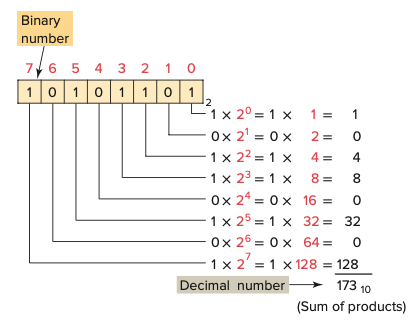
\includegraphics[width = 0.4\textwidth]{2_images/int.png}
            \caption{An 8 bit integer \cite{petruzella2017programmable}.}
            \label{fig:int}
        \end{figure}         

\section{Communication}

\subsection{Serial}
    Serial communication is a method of data transfer between devices where data is transmitted and received one "bit" at a time \cite{frenzel2015handbook}. Communication is typically facilitated through copper wires where data is represented by electrical signals. Serial communication standards define the specifics as to exactly how the data is transferred and interpreted. Below are some basic descriptions of a few common terms used within serial communication.
    
    \begin{description}
    
    \item[Baud Rate] The baud rate refers to the speed of data transfer. More specifically it refers to how many bits are able to be transmitted and received per second. 
    
    \item[Communication Mode] There are three different types of communication modes: Simplex, Half Duplex and Full Duplex. For the sake of simplicity, the following explanations are in reference to a peer-to-peer system comprising of only two devices, lets call them Device-A and Device-B. Simplex means that communication is one way - Device-A is capable of transmitting data while device-B is capable of only receiving data.
    
    \item[Asynchronous/ Synchronous] Data transmission can be achieved through either synchronous or asynchronous methods of communication. \HD{Explain the differences and don't forget to reference.}
    
    \end{description}
    
    The lolly machine utilises three flavours of serial communication, these are as follows.
    
    \subsubsection{RS-232}
    RS-232 has been around for a long time and is one of the older methods of serial communication. Although there are many superior methods of communication in this modern era, RS-232 is still common among industry. 
    RS-232 is supported by the Click \acrshort{plc}. During normal operation, the \acrshort{plc} communicates to all system peripherals through an Ethernet protocol and does not require RS-232. Unfortunately, the \acrshort{plc} factory settings do not include a static \acrshort{ip}\footnote{An \acrshort{ip} address is a unique address required for the type of communication network (router-less Ethernet) that that has been implemented on the lolly machine} address.  RS-232 is used exclusively for setting the \acrshort{ip} address of the \acrshort{plc}. Figure \ref{fig:rs232Trans} shows a typical RS-232 data transmission. 

    \begin{figure}[H]
        \centering
        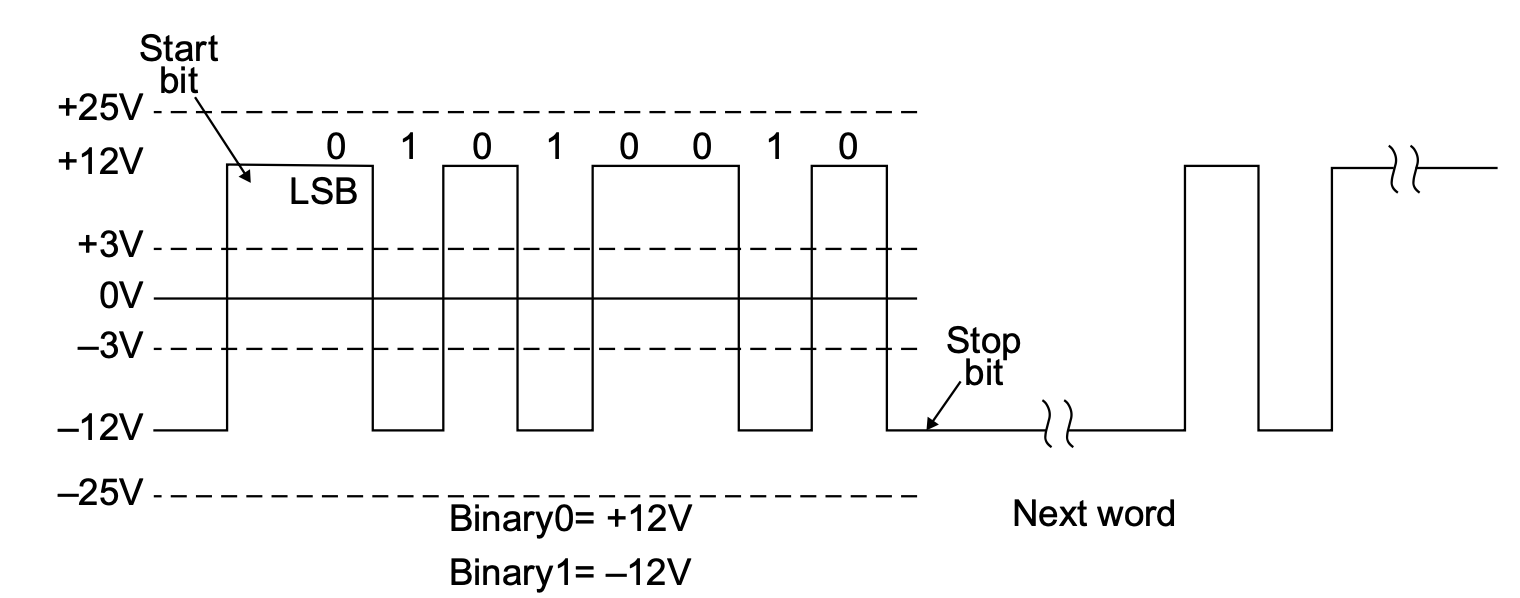
\includegraphics[width = 0.7\textwidth]{2_images/rs232Trans.png}
        \caption{A RS-232 data transmission~\cite{frenzel2015handbook}.}
        \label{fig:rs232Trans}
    \end{figure}   
    
    \subsubsection{RS-485}
    The RS-485 serial protocol is used for communication between the Arduino and the \acrshort{plc}.
    
    \subsubsection{SPI}
    The SPI protocol is used to link the Arduino to the \acrshort{rgb} \acrshort{led}s.
    
    % could also include spi and i2c but we will see. . . 

 
     
\subsection{Ethernet}
    Ethernet, also known as IEEE 802.3, is a commonly used communication standard that governs the Physical and Data-Link Link layers (in relation to the \acrshort{osi}\footnote{The \acrshort{osi} model provides a framework that describes how applications can communicate over a wired \acrshort{lan}\cite{scott2021networking}.} model shown in Figure \ref{fig:osi}) of a wired \acrshort{lan}\cite{scott2021networking}. A wired \acrfull{lan} is a group of network devices that are connected on a local Ethernet network.  
    
        \begin{figure}[H]
            \centering
            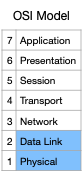
\includegraphics[width = 0.1\textwidth]{2_images/osi.png}
            \caption{The \acrshort{osi} model\cite{scott2021networking}.}
            \label{fig:osi}
        \end{figure} 
    
    An Ethernet network is established through physical cabling. Cabling can be coaxial, twisted copper pairs of fibre optic \cite{scott2021networking}.
    
    All devices on the lolly machine support Ethernet, subsequently all devices are on the same \acrshort{lan}.
    
    Each Ethernet device has a unique address which is called an \acrshort{ip} address. An \acrshort{ip} address is a four-octet, eight-bit address\cite{scott2021networking}.  
    
    \begin{figure}[H]
        \centering
        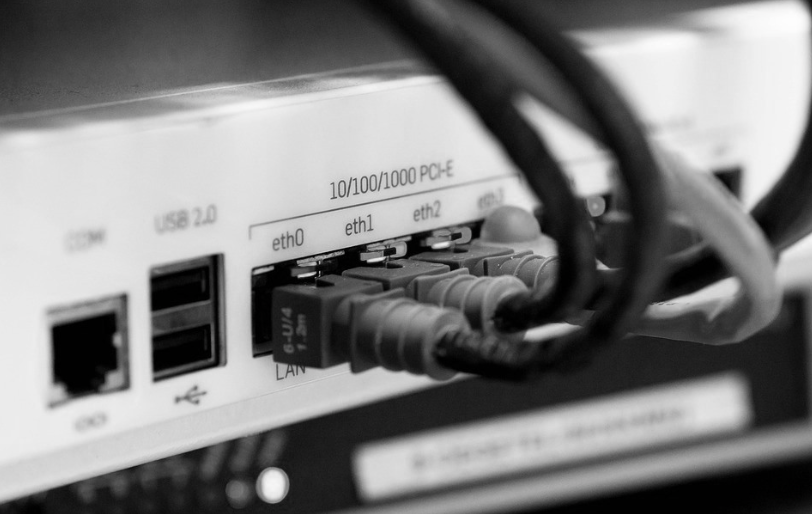
\includegraphics[width = 0.6\textwidth]{2_images/ethernetCables.png}
        \caption{Ethernet cables plugged into a network switch\cite{scott2021networking}.}
        \label{fig:ethenetCables}
    \end{figure} 

    There are two main types of Ethernet devices - Client device and Server device. To best explain the relationship between Client and Server devices, the following analogy can be used. In a restaurant, the customer requests food from the waiter. The waiter listens to the customers request and proceeds to deliver the food back to the customer. If you haven't already guessed, the customer is the Client, the waiter is the Server and the food is data. This is similar to the a Master/ Slave relationship in serial networks where the Master is the Client and the Slave is the Server. It is not uncommon for devices to be both Clients and Servers, these types of devices are referred to as a Client-Server device.
    
        
\section{Communication Protocols}
\subsection{Modbus}
    Modbus is an open-source \footnote{Open-source means that the developers have made the protocol available to the public. This allows third parties to use the protocol in their own products.} communication protocol that was produced by Modicon \cite{frenzel2015handbook}. Modbus was originally used exclusively in serial networks (RS-232 and RS-485) but has now expanded to TCP/IP which runs over an Ethernet network\cite{frenzel2015handbook}. 
    
    There are two main types of devices in a Modbus network, the Master and Slave\cite{frenzel2015handbook}. The Master can request data from a slave but not vice versa. A Master cannot request data from another master and a slave cannot request data another slave. Some devices like \acrshort{plc}s can be Mater/Slaves allowing inter \acrshort{plc} communication and tiered hierarchy of control. E.g., the \acrshort{hmi} on the lolly machine controls the \acrshort{plc} and the \acrshort{plc} controls the remote \acrshort{io}. Modbus on an Ethernet network operates on the same principles as those describe above however, the terminology is slightly different. A Master device is referred to as a Client while a Slave device is referred to as a Server. A way to remember this is that a server "serves" the client.
    
    In a Modbus network, data is communicated between devices in single bits or in WORDs (2 BYTES). 
    The Modbus protocol has four different address types, these are as follows:
    
        \begin{table}[H]
        \caption{Modbus Address Types}
        \begin{center}
            \begin{tabular}{ |c|c|c| }
                \hline
                \textbf{Data Type} & \textbf{Size} & \textbf{Access}\\ 
                \hline
                Coil                & 1 Bit         & Read/ Write Access\\
                Discrete Input      & 1 bit         & Read only Access\\
                Input Register      & 16 bit (WORD) & Read only Access\\
                Holding Register        & 16 bit (WORD) & Read/ Write Access\\
                \hline
            \end{tabular}\\
        \end{center}
        \label{table:modbusAddressTypes}
    \end{table}
    
    When the Master/ Client device requests data from the Slave/ Server, it does so with a function code. The function code lets the Slave/ Server know how to respond to the request. The below list shows what each code corresponds to. 

    \begin{table}[H]
        \caption{Modbus Functions}
        \begin{center}
            \begin{tabular}{ |c|c| }
                \hline
                \textbf{Code} & \textbf{Name}\\ 
                \hline
                01 & Read Coil Status\\
                02 & Read Input Status\\
                03 & Read Holding Registers\\
                04 & Read Input Registers\\
                05 & Force Single Coil\\
                06 & Preset Single Register\\
                07 & Read Exception Status\\
                08 & Diagnostics\\
                09 & Program 484\\
                10 & Poll 484\\
                11 & Fetch Comm. Event Ctr\\
                12 & Fetch Comm. Event Log\\
                13 & Program Controller\\
                14 & Poll Controller\\
                15 & Force Multiple Coils\\
                16 & Preset Multiple Registers\\
                17 & Report Slave ID\\
                18 & Program 884/M84\\
                19 & Reset Comm. Link\\
                20 & Read General Reference\\
                21 & Write General Reference\\
                \hline
            \end{tabular}\\
        \end{center}
        \label{table:modbusFunctions}
    \end{table}

The Modbus TCP/IP communication protocol is used extensively throughout various components of the lolly machine. Figure \ref{fig:networkArcitecture} shows how the Modbus communication protocol facilitates the overall network architecture of the project.
